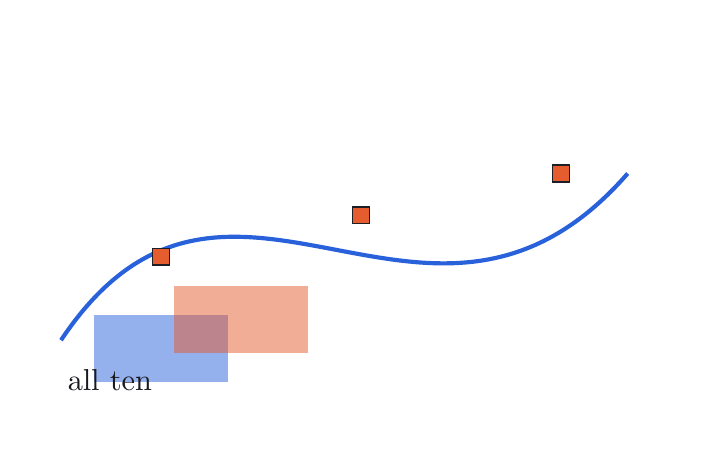
\begin{tikzpicture}[every node/.style={inner sep=0bp,outer sep=0bp}]
  \definecolor{qcA}{rgb}{0.16,0.38,0.86}
  \def\mareymarkB#1#2{\path[fill,draw,shift={(#1,#2)}] (-3bp,-3bp) rectangle (3bp,3bp);}
  \definecolor{qcC}{rgb}{0.9,0.36,0.18}
  \definecolor{qcD}{rgb}{0.11,0.12,0.15}
  \definecolor{qcE}{rgb}{0.1,0.1,0.12}
  \useasboundingbox (0bp,0bp) rectangle (240bp,150bp);
  % marey-key: all-ten
  % marey-role: series -- everything
  % marey-data: cases = 10
  \begin{scope}
    \clip (4.8bp,10.5bp) -- (235.2bp,10.5bp) -- (235.2bp,142.5bp) -- (4.8bp,142.5bp) -- cycle;
    \path[draw=qcA,line width=1.5bp] (12bp,37.5bp) .. controls (72bp,127.5bp) and (144bp,15bp) .. (216bp,97.5bp);
    \begin{scope}[fill=qcC,draw=qcD,line width=0.563bp]
      \mareymarkB{48bp}{67.5bp}
      \mareymarkB{120bp}{82.5bp}
      \mareymarkB{192bp}{97.5bp}
    \end{scope}
    \path[fill=qcA,fill opacity=0.5] (24bp,22.5bp) -- (72bp,22.5bp) -- (72bp,46.5bp) -- (24bp,46.5bp) -- cycle;
    \path[fill=qcC,fill opacity=0.5] (52.8bp,33bp) -- (100.8bp,33bp) -- (100.8bp,57bp) -- (52.8bp,57bp) -- cycle;
    \node[anchor=base west,text=qcE,font=\fontsize{11}{13.2}\selectfont] at (14.4bp,19.5bp) {all ten};
  \end{scope}
\end{tikzpicture}
